% CO3133 - Assignment 3 Milestone 2 (scientific draft)
% Editable, single-source XeLaTeX manuscript. Charts and confusion matrix use
% PGFPlots/TikZ; all data labels are grounded in the archived 9 real M2 dev runs.
% Compile: xelatex -interaction=nonstopmode -halt-on-error main.tex (twice)
\documentclass[11pt,a4paper]{article}

% --- Typography and page construction (conservative academic style) ---
\usepackage[a4paper,left=23mm,right=23mm,top=23mm,bottom=22mm,headheight=14pt,headsep=7mm,footskip=11mm]{geometry}
\usepackage{fontspec}
\IfFileExists{/usr/share/fonts/truetype/liberation/LiberationSerif-Regular.ttf}{%
  \setmainfont[Path=/usr/share/fonts/truetype/liberation/,
    BoldFont=LiberationSerif-Bold.ttf,
    ItalicFont=LiberationSerif-Italic.ttf,
    BoldItalicFont=LiberationSerif-BoldItalic.ttf]{LiberationSerif-Regular.ttf}%
}{\setmainfont{TeX Gyre Termes}}
\usepackage{unicode-math}
\IfFileExists{/usr/share/texmf/fonts/opentype/public/lm-math/latinmodern-math.otf}{%
  \setmathfont[Path=/usr/share/texmf/fonts/opentype/public/lm-math/]{latinmodern-math.otf}%
}{\setmathfont{Latin Modern Math}}
\usepackage{microtype}
\usepackage{setspace}
\setstretch{1.055}
\usepackage{amsmath}
\usepackage{booktabs,tabularx,array,multirow,longtable}
\usepackage{caption}
\captionsetup{font=small,labelfont=bf,justification=justified,singlelinecheck=false,skip=5pt}
\usepackage{titlesec}
\titleformat{\section}{\fontsize{12}{14}\selectfont\bfseries}{\thesection.}{0.6em}{}
\titleformat{\subsection}{\fontsize{11}{13}\selectfont\bfseries}{\thesubsection}{0.7em}{}
\titlespacing*{\section}{0pt}{11pt}{5pt}
\titlespacing*{\subsection}{0pt}{8pt}{3pt}
\usepackage{fancyhdr}
\pagestyle{fancy}
\fancyhf{}
\fancyhead[L]{\footnotesize CO3133 \;|\; Group Goat \;|\; Assignment 3 -- Milestone 2}
\fancyhead[R]{\footnotesize Experimental draft}
\fancyfoot[L]{\footnotesize 17 November 2026}
\fancyfoot[R]{\footnotesize Page \thepage}
\renewcommand{\headrulewidth}{0.3pt}
\renewcommand{\footrulewidth}{0pt}
\setlength{\parindent}{0pt}
\setlength{\parskip}{3.0pt plus 0.6pt minus 0.3pt}
\setlength{\tabcolsep}{5.1pt}
\renewcommand{\arraystretch}{1.12}
\usepackage{enumitem}
\setlist{nosep,leftmargin=1.5em}
\usepackage{float}
\usepackage[section]{placeins}
\usepackage{xcolor}
\definecolor{imageblue}{HTML}{4477AA}
\definecolor{textorange}{HTML}{CC6677}
\definecolor{fusionteal}{HTML}{009988}
\definecolor{heatblue}{HTML}{2D63AA}
\definecolor{gridgray}{HTML}{D6DCE2}
\usepackage{tikz}
\usepackage{pgfplots}
\pgfplotsset{compat=1.18}
\usepgfplotslibrary{groupplots}
\usetikzlibrary{calc,positioning}
\usepackage[hidelinks]{hyperref}
\usepackage{xurl}
\urlstyle{same}
\usepackage{lastpage}

\newcommand{\dev}{\textit{development}}
\newcommand{\trn}{\textit{training}}
\newcommand{\tst}{\textit{test}}
\newcommand{\primary}{\texttt{filtered\_original}}
\newcommand{\smallnote}[1]{\par\vspace{-4pt}{\footnotesize\itshape #1}\par}
\newcommand{\HeadRule}{\noalign{\global\arrayrulewidth=0.4pt}\midrule}

\begin{document}
\begin{center}
{\footnotesize\bfseries HO CHI MINH CITY UNIVERSITY OF TECHNOLOGY -- VNU-HCM}\\[2pt]
{\footnotesize Faculty of Computer Science and Engineering \;|\; Deep Learning and Its Applications (CO3133)}\\[2pt]
{\footnotesize Semester 261 \;|\; Instructor: Lê Thành Sách}\\[13pt]
{\Large\bfseries Humanitarian Image--Text Classification with\\[2pt]
Frozen Encoders and Concatenation Fusion}\\[7pt]
{\normalsize\bfseries Assignment 3, Milestone 2 -- Experimental Draft Report}\\[5pt]
{\normalsize Group Goat}\\[3pt]
{\small Nguyễn Huỳnh Nam Quốc (2453089) -- Assignment 3 lead, 100\% contribution}\\[2pt]
{\small Hoàng Trọng Huy Minh (2452743), 0\% \;|\; Võ Lê Thành Triệu (2453297), 0\%}\\[3pt]
{\small 17 November 2026}
\end{center}
\vspace{6pt}

\noindent{\bfseries Abstract.}\;
This draft investigates five-class humanitarian classification of paired crisis-related images and tweets on an explicitly mirror-derived, leakage-filtered subset of CrisisMMD v2.0. Following a locked Milestone 1 (M1) protocol, 7,938 aligned image--text records are retained (6,001 training, 986 development, and 951 held-out test records). Frozen ImageNet-pretrained ResNet-18 and DistilBERT encoders produce 512- and 768-dimensional features, respectively. We compare an image-only head, a text-only head, and a simple concatenation fusion head under matched training settings and three random seeds (42, 43, 44). On the development set, mean macro-F1 (sample standard deviation) is 0.5746 (0.0068), 0.6811 (0.0016), and 0.8116 (0.0041), respectively; the corresponding mean accuracies are 69.30\%, 77.62\%, and 85.40\%. The fusion head exceeds the stronger unimodal baseline by 0.1305 macro-F1 on these development runs. Reported numbers were recomputed from saved predictions; all nine checkpoints reproduced their saved development predictions in an earlier verification. Results remain development-only and establish neither held-out test performance nor unseen-disaster or deployment generalization.

{\footnotesize\textbf{Keywords:} multimodal learning; CrisisMMD; humanitarian classification; feature fusion; macro-F1; reproducibility.}

\section{Introduction}
Crisis-related social-media posts often combine text and imagery. The two modalities can encode distinct but related evidence about damaged infrastructure, affected people, rescue activities, and non-humanitarian content. CrisisMMD was introduced to support multimodal disaster-information research \cite{alam2018}. This study asks whether concatenating pretrained image and text representations improves classification relative to either modality alone while holding the underlying paired records, partition membership, optimization settings, loss, and seeds fixed.

Milestone 2 (M2) is an intermediate graded checkpoint, not the final Assignment 3 report. In accordance with the course handbook \cite{handbook2026}, M2 covers two unimodal models and a simple fusion baseline with quantitative evidence. Learned gated fusion, controlled fusion ablation, semantic support/conflict case review, and held-out model evaluation are reserved for M3. No M3 training or test-set prediction is reported here.

\section{Dataset and Integrity Controls}
\subsection{Source, task, and prediction unit}
The source is a custom five-class agreed-label humanitarian derivative of QCRI CrisisMMD v2.0, accessed through the pinned third-party \texttt{pranitchawla/crisismmd-mteb} mirror.\footnote{Pinned mirror revision: \texttt{a935fda3cee8a5250746a8d1d6278214d615cc89}.} The dataset version is \texttt{crisismmd5-mirror-remediation-20261104-v1}; the primary protocol is \primary. The prediction unit is one image attached to one tweet; a single tweet may contribute multiple image records. The retained pairs represent the corpus's historical disaster-event mixture, not an unseen-event benchmark. License and derivative attribution follow CC BY-NC-SA 4.0 \cite{qcri2026,mirror2026}; no raw media or tweet text is reproduced in this document.

\subsection{Locked partitions and class distribution}
\begin{table}[htbp]
\centering\small
\caption{Locked class counts in \primary. The held-out partition is documented for provenance only; M2 model evaluation uses development data.}
\label{tab:classcounts}
\begin{tabularx}{\linewidth}{@{}>{\raggedright\arraybackslash}Xrrrr@{}}
\toprule
Humanitarian class (ID) & Train & Dev & Test & Total \\
\midrule
Affected individuals (0) & 71 & 9 & 9 & 89 \\
Infrastructure and utility damage (1) & 601 & 80 & 81 & 762 \\
Rescue volunteering/donation (2) & 901 & 148 & 126 & 1,175 \\
Other relevant information (3) & 1,247 & 235 & 235 & 1,717 \\
Not humanitarian (4) & 3,181 & 514 & 500 & 4,195 \\
\midrule
\textbf{Total} & \textbf{6,001} & \textbf{986} & \textbf{951} & \textbf{7,938} \\
\bottomrule
\end{tabularx}
\end{table}
The initial audit pool comprised 8,079 records. M1 remediation excluded 7 unresolved source-label discrepancies, 9 verified placeholders, and 125 lower-priority duplicate/leakage-related records. Transitive grouping relied on tweet identities, byte/pixel image hashes, raw/normalized text hashes, and reviewed duplicate edges. When a group crossed source splits, retention followed test $>$ dev $>$ train without moving retained observations. These decisions were locked \emph{before} M2 and were not changed in response to model scores. The full split manifests and their SHA-256 locks are in the published M1 repository \cite{handbook2026}.

The cached splits contain 5,139 distinct training groups, 983 development groups, and 949 held-out groups. Within-split record IDs were checked for uniqueness. The affected-individuals class has only nine development examples; this directly limits the stability of its class-specific estimates. Grouping reduces observed identity/duplicate leakage but cannot prove the absence of every possible semantic duplicate.

\subsection{Paired input checks and diagnostics}
Each retained image--text pair was linked to a fixed image ID, tweet ID, event, label, and audited content hashes prior to encoder extraction. The original 8,079-pair audit found no empty source text and no corrupt source images; nine decodable placeholders were later excluded. Preliminary source-pool texts had a median of 14 whitespace-delimited words (95th percentile 20), which should not be confused with tokenization statistics from the filtered sample.

Across the 7,938 retained pairs, the actual DistilBERT tokenizer pass produced mean length 17.14 subtokens, maximum length 81, no truncation at the 128-subtoken limit, and 19 unknown-token occurrences. These measurements show tokenization behavior, not a population-level estimate of semantic image--text correspondence.

\section{Methods}
\subsection{Frozen feature-extraction pipeline}
RGB images were processed with the official \texttt{ResNet18\_Weights.IMAGENET1K\_V1} inference recipe: resize shorter side to 256, center-crop to $224\times224$, and apply ImageNet normalization \cite{he2016,torchvision2026}. Removing the pretrained classification layer yielded a fixed 512-dimensional image representation $\mathbf{v}_i\in\mathbb{R}^{512}$. Tweets were normalized using HTML unescaping, Unicode NFKC, case folding, and URL/mention removal before tokenization. The pinned \texttt{distilbert-base-uncased} encoder (commit \texttt{12040accade4e8a0f71eabdb}\allowbreak\texttt{258fecc2e7e948be}) generated masked-mean-pooled token features $\mathbf{v}_t\in\mathbb{R}^{768}$ \cite{sanh2019,distilbert2026}.

Both encoders operated in inference mode and were frozen throughout M2. Record IDs align the two cached feature matrices; encoder finetuning was not performed. This design limits computational cost and isolates the comparison to the learned classification heads and fusion operation.

\subsection{Image-only, text-only, and concatenation heads}
For each modality $m\in\{i,t\}$, a trainable projection maps the frozen feature $\mathbf{v}_m$ to $\mathbf{h}_m=\operatorname{ReLU}(W_m\mathbf{v}_m+b_m)\in\mathbb{R}^{128}$. A unimodal model applies dropout ($p=0.2$) followed by a five-logit linear classifier. The simple multimodal baseline concatenates the two projected vectors and applies a further 128-unit ReLU hidden layer, dropout, and five-logit output:
\begin{equation}
\mathbf{z}_{\mathrm{concat}} = W_o\,\mathrm{Dropout}\!\left(\operatorname{ReLU}\!\left(W_f[\mathrm{Dropout}(\mathbf{h}_i);\,\mathrm{Dropout}(\mathbf{h}_t)]+b_f\right)\right)+b_o.
\label{eq:fusion}
\end{equation}
All heads use weighted cross-entropy on the shared five-class pair label, with no auxiliary modality loss for concatenation.

\begin{table}[htbp]
\centering\small
\caption{Implemented M2 classification heads; parameter counts exclude the frozen pretrained encoders.}
\label{tab:models}
\begin{tabularx}{\linewidth}{@{}l>{\raggedright\arraybackslash}X>{\raggedright\arraybackslash}Xr@{}}
\toprule
Configuration & Frozen source & Trainable head & Parameters \\
\midrule
Image only & ResNet-18 (512-D) & $512\to128\to5$ & 66,309 \\
Text only & DistilBERT (768-D) & $768\to128\to5$ & 99,077 \\
Concatenation & Both (512-D + 768-D) & $512/768\to128$ each; concat 256; $128\to5$ & 197,637 \\
\bottomrule
\end{tabularx}
\end{table}

\subsection{Optimization, model selection, and metrics}
Each architecture was trained with seeds $\{42,43,44\}$, Adam optimizer, learning rate $10^{-3}$, weight decay $10^{-4}$, batch size 64, and a maximum of 30 epochs. Class weights were computed \emph{only} from the 6,001 training labels: initial $w_c=N_{\mathrm{train}}/(5n_c)$, subsequently normalized to mean one. A common weighted cross-entropy loss controlled class imbalance.

Checkpoint selection maximized development macro-F1 with patience five. Tied macro-F1 values were resolved by lower development loss, and then the earlier epoch. Best checkpoints were reloaded for the recorded predictions. Primary metric is macro-F1:
\begin{equation}
\mathrm{MacroF1}=\frac{1}{5}\sum_{c=0}^{4}\frac{2P_cR_c}{P_c+R_c},\qquad
\mathrm{Accuracy}=\frac{\#\text{ correct dev predictions}}{986},
\end{equation}
where zero-denominator class-F1 follows the implementation's zero convention. Accuracy, per-class precision/recall/F1, and raw/row-normalized $5\times5$ confusion matrices were computed on the same development predictions. The reported SD is the \emph{sample} standard deviation of three seed results, not a confidence interval for unseen events. The held-out test set did not enter M2 training, checkpoint selection, or quantitative reporting.

\section{Experimental Setup and Verification}
Real execution took place on Google Colab with an NVIDIA Tesla T4 GPU (15 GiB VRAM), Python 3.13.16, PyTorch 2.14.1+cu130, torchvision 0.29.1+cu130, transformers 4.57.6, and pyarrow 23.0.1. Frozen feature extraction of the 7,938 pairs took 144.66 s in the recorded run. This includes model loading and potentially initial cache/network preparation; it should not be interpreted as an isolated GPU-only throughput measurement.

The feature cache consists of \texttt{train.npz}, \texttt{dev.npz}, and \texttt{test.npz} (512 image and 768 text dimensions per record), accompanied by per-file SHA-256 fingerprints, IDs, group labels, and membership checks. The held-out cache was produced for later work but was not used for M2 model comparison. Nine run directories each contain \texttt{best.pt}, \texttt{run.json}, and \texttt{dev\_predictions.csv}.

A prior independent verification loaded every checkpoint, reconstructed the associated CPU head, and regenerated predictions for all 986 development records; each matched its saved prediction CSV exactly (9 of 9). Accuracy, macro-F1, class-level scores, and confusion matrices were recomputed from those files and matched saved run metadata. This confirms internal artifact consistency, but is \emph{not} a separate end-to-end reproduction of feature extraction from raw image and text bytes.

\section{Development Results}
\subsection{Quantitative comparison}
\begin{table}[htbp]
\centering\small
\caption{Mean $\pm$ sample SD over three M2 development runs per model. Training times sum head fitting and dev checkpoint selection only; common encoder extraction is excluded.}
\label{tab:mainresults}
\begin{tabularx}{\linewidth}{@{}l>{\centering\arraybackslash}X>{\centering\arraybackslash}Xrr@{}}
\toprule
Model & Dev macro-F1 & Dev accuracy & Head time (s) & Trainable params \\
\midrule
Image only & $0.5746\pm0.0068$ & $69.30\%\pm0.77$ pp & 12.69 & 66,309 \\
Text only & $0.6811\pm0.0016$ & $77.62\%\pm0.64$ pp & 10.49 & 99,077 \\
\textbf{Concatenation} & $\mathbf{0.8116\pm0.0041}$ & $\mathbf{85.40\%\pm0.44}$ pp & 18.91 & 197,637 \\
\bottomrule
\end{tabularx}
\end{table}
Concatenation attains 0.8116 macro-F1, compared with 0.6811 for text only and 0.5746 for image only. Its mean development advantage is $+0.1305$ macro-F1 over text and $+0.2370$ over image; mean accuracy is higher by 7.78 and 16.09 percentage points, respectively. Between-seed variation on this fixed development set is small, but does not establish statistical significance under changes in event distribution or source population.

\subsection{Per-class behavior}
\begin{table}[htbp]
\centering\small
\caption{Class-wise development F1 averaged over seeds 42, 43, 44. Support is unchanged across runs; all values are descriptive.}
\label{tab:perclass}
\begin{tabularx}{\linewidth}{@{}>{\raggedright\arraybackslash}Xrrrr@{}}
\toprule
Class & Support & Image F1 & Text F1 & Concat F1 \\
\midrule
0: Affected individuals & 9 & 0.116 & 0.378 & 0.679 \\
1: Infrastructure damage & 80 & 0.651 & 0.713 & 0.838 \\
2: Rescue/donation effort & 148 & 0.627 & 0.760 & 0.839 \\
3: Other relevant & 235 & 0.747 & 0.720 & 0.822 \\
4: Not humanitarian & 514 & 0.733 & 0.836 & 0.881 \\
\bottomrule
\end{tabularx}
\end{table}

\begin{figure}[htbp]
\centering
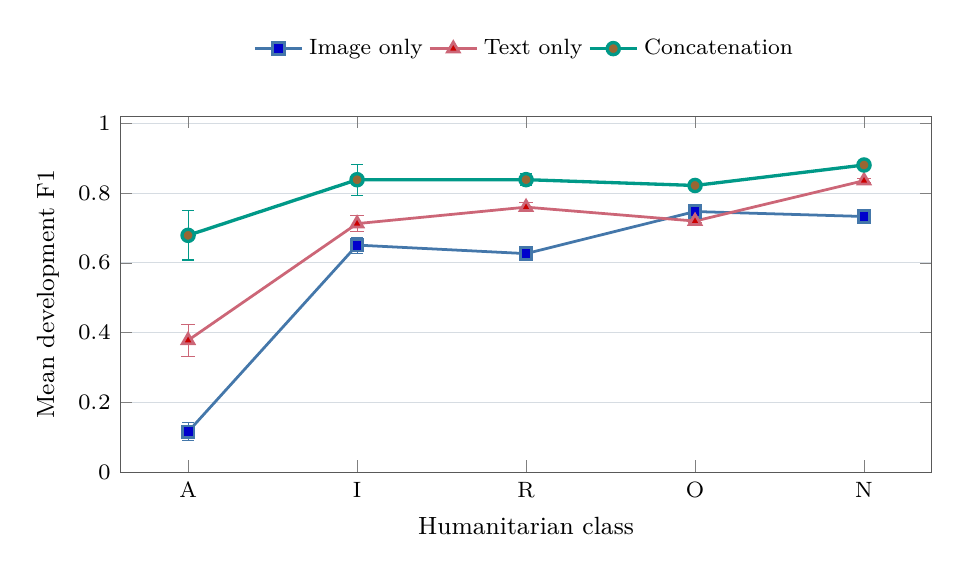
\begin{tikzpicture}
\begin{axis}[
  width=0.98\linewidth,height=6.1cm,
  ymin=0,ymax=1.02,
  ylabel={Mean development F1},xlabel={Humanitarian class},
  xtick={0,1,2,3,4},xticklabels={A,I,R,O,N},
  ymajorgrids,grid style={draw=gridgray,thin},
  axis line style={black!65},tick label style={font=\footnotesize},
  label style={font=\small},
  legend style={draw=none,at={(0.5,1.13)},anchor=south,legend columns=3,font=\footnotesize},
  error bars/y dir=both,error bars/y explicit,
  ]
\addplot+[color=imageblue,mark=square*,line width=1pt,mark size=2.1pt] coordinates {
 (0,0.1158) +- (0,0.0253) (1,0.6509) +- (0,0.0229) (2,0.6265) +- (0,0.0081) (3,0.7471) +- (0,0.0149) (4,0.7329) +- (0,0.0173)};
\addlegendentry{Image only}
\addplot+[color=textorange,mark=triangle*,line width=1pt,mark size=2.4pt] coordinates {
 (0,0.3779) +- (0,0.0453) (1,0.7125) +- (0,0.0238) (2,0.7597) +- (0,0.0133) (3,0.7198) +- (0,0.0039) (4,0.8356) +- (0,0.0067)};
\addlegendentry{Text only}
\addplot+[color=fusionteal,mark=*,line width=1.2pt,mark size=2.2pt] coordinates {
 (0,0.6789) +- (0,0.0708) (1,0.8383) +- (0,0.0441) (2,0.8385) +- (0,0.0180) (3,0.8218) +- (0,0.0047) (4,0.8805) +- (0,0.0025)};
\addlegendentry{Concatenation}
\end{axis}
\end{tikzpicture}
\caption{Mean class-specific development F1 $\pm$ sample SD over three seeds. Labels: A = affected individuals, I = infrastructure damage, R = rescue/donation effort, O = other relevant, N = not humanitarian. Colored series distinguish the models; comparisons are confined to dev.}
\label{fig:classf1}
\end{figure}

Fusion improves the mean class-level F1 over the stronger unimodal result for all five classes (Table~\ref{tab:perclass}; Figure~\ref{fig:classf1}). The largest descriptive gap occurs for affected individuals: 0.116 (image), 0.378 (text), and 0.679 (fusion). Because there are only nine development observations for this class, a single change in true-positive recall corresponds to 11.1 percentage points; this apparent improvement is promising but unstable.

\subsection{Fusion confusion matrix}
\begin{figure}[htbp]
\centering
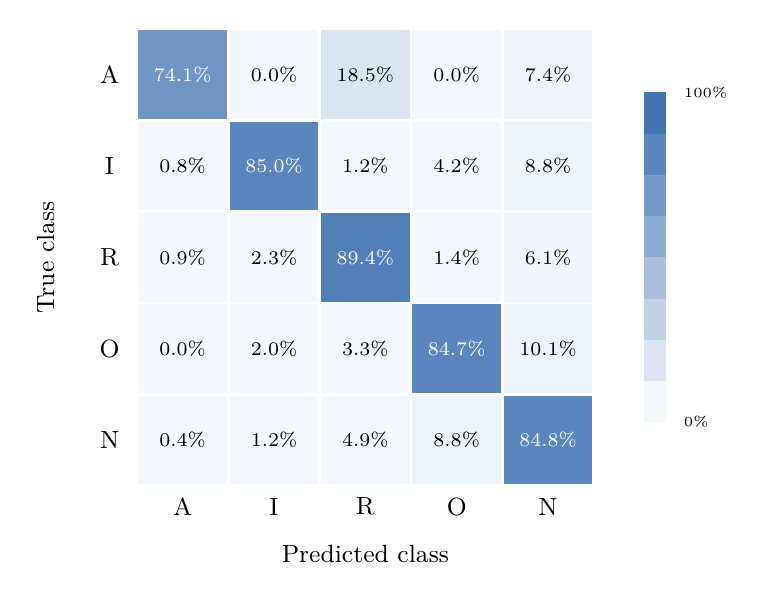
\begin{tikzpicture}[x=1.16cm,y=1.16cm]
% Heat intensity is normalized to percentage; white->blue gradient.
\newcommand{\heatcell}[3]{%
  \pgfmathtruncatemacro{\shaden}{max(5,min(90,round(#3*0.92)))}%
  \path[fill=heatblue!\shaden!white,draw=white,line width=1pt] (#1,{4-#2}) rectangle ++(1,1);%
  \ifnum\shaden>55
    \node[font=\scriptsize,text=white] at ({#1+0.5},{4.5-#2}) {#3\%};%
  \else
    \node[font=\scriptsize,text=black] at ({#1+0.5},{4.5-#2}) {#3\%};%
  \fi
}
\heatcell{0}{0}{74.1}\heatcell{1}{0}{0.0}\heatcell{2}{0}{18.5}\heatcell{3}{0}{0.0}\heatcell{4}{0}{7.4}
\heatcell{0}{1}{0.8}\heatcell{1}{1}{85.0}\heatcell{2}{1}{1.2}\heatcell{3}{1}{4.2}\heatcell{4}{1}{8.8}
\heatcell{0}{2}{0.9}\heatcell{1}{2}{2.3}\heatcell{2}{2}{89.4}\heatcell{3}{2}{1.4}\heatcell{4}{2}{6.1}
\heatcell{0}{3}{0.0}\heatcell{1}{3}{2.0}\heatcell{2}{3}{3.3}\heatcell{3}{3}{84.7}\heatcell{4}{3}{10.1}
\heatcell{0}{4}{0.4}\heatcell{1}{4}{1.2}\heatcell{2}{4}{4.9}\heatcell{3}{4}{8.8}\heatcell{4}{4}{84.8}
\foreach \name [count=\ix from 0] in {A,I,R,O,N}{
  \node[font=\small] at ({\ix+0.5},-0.23) {\name};
  \node[font=\small] at (-0.30,{4.5-\ix}) {\name};
}
\node[font=\small] at (2.5,-0.75) {Predicted class};
\node[font=\small,rotate=90] at (-1.00,2.5) {True class};
% compact swatches to communicate continuous intensity; approximate gradient by 8 steps
\foreach \k in {0,...,7}{\pgfmathsetmacro{\level}{round(5+85*\k/7)}\path[fill=heatblue!\level!white,draw=none] (5.55,{0.70+0.45*\k}) rectangle ++(0.24,0.46);}
\node[font=\tiny,anchor=west] at (5.88,0.70) {0\%};
\node[font=\tiny,anchor=west] at (5.88,4.30) {100\%};
\end{tikzpicture}
\caption{Row-normalized concatenation confusion matrix, computed by averaging percentages across three development seeds. Cells give $P(\widehat{y}=j\mid y=i)$ in percent; displayed values are rounded. Class abbreviations follow Figure~\ref{fig:classf1}. The held-out test set is not shown.}
\label{fig:confusion}
\end{figure}

The most frequent residual off-diagonal fusion confusion is from not-humanitarian (N) to other relevant information (O), averaging 45 out of 514 cases per seed (8.8\%). The reverse O-to-N error averages 23.7 out of 235 (10.1\%). Figure~\ref{fig:confusion} visualizes the full row-normalized pattern and supports a more nuanced interpretation than accuracy alone.

\subsection{Paired development predictions}
\begin{table}[htbp]
\centering\small
\caption{Paired dev prediction patterns (identical 986 records per seed). These operational categories do not establish semantic agreement or conflict in raw paired media.}
\label{tab:paired}
\begin{tabularx}{\linewidth}{@{}>{\raggedright\arraybackslash}Xrrr@{}}
\toprule
Pattern & Seed 42 & Seed 43 & Seed 44 \\
\midrule
Unimodal predictions disagree & 386 & 382 & 373 \\
Fusion correct despite both unimodal heads incorrect & 16 & 28 & 20 \\
Fusion correct when image incorrect, text correct & 184 & 168 & 161 \\
Fusion correct when image correct, text incorrect & 95 & 95 & 91 \\
Fusion incorrect despite at least one unimodal correct & 59 & 71 & 73 \\
\bottomrule
\end{tabularx}
\end{table}

For seed 42 the unimodal heads disagree on 386/986 observations. Concatenation correctly classifies 294 such disagreements, but incorrectly classifies 59 records on which at least one unimodal classifier is correct. It also recovers 16 records for which both unimodal predictions are wrong. The pattern of recoveries and harms occurs in all three seeds. These are \emph{prediction-based} complementarity and conflict patterns; confirming semantic modality support/conflict would require reviewing the original image and text pairs, which is not claimed in M2.

\section{Compute Accounting and Limitations}
Shared frozen-encoder extraction took 144.66 s and was reused by the nine head-training runs. Cumulative head-training-plus-dev-selection time was 42.09 s, comprising 12.69 s (image), 10.49 s (text), and 18.91 s (concatenation). These are measured run-specific quantities, not separate end-to-end training costs per configuration. Roughly 0.003 s recorded per dev head-only prediction pass does not include decoding, tokenizer work, or encoder inference and cannot be presented as deployable latency. Peak GPU memory, energy use, and a standardized batch-controlled end-to-end latency experiment were not logged.

Four constraints bound interpretation. First, \primary{} is custom-filtered from a third-party mirror; byte-for-byte equivalence with the original official agreed-label archive remains unverified. Second, source disaster events overlap train and dev, preventing claims about unseen-disaster generalization. Third, the agreed-label corpus may underrepresent naturally conflicting image--text observations, while metadata linkage alone cannot establish semantic truth for every pair. Fourth, 9/986 dev observations belong to class 0 and 514/986 to class 4, sharply limiting rare-class inference in an imbalanced setting. Dev scores must not be used to select a single best seed for test reporting or to assert deployment readiness.

\section{Reproducibility and M2 Completion Scope}
Evidence supplied for this draft includes nine checkpoint directories (one per model and seed), per-run training histories and dev predictions, summary CSVs, and three locked feature caches. The core script entry points are \path{m2m3/run_all.py --milestone m2} and \path{m2m3/summarize_dev.py --milestone m2}; their sources are preserved in the separate implementation package. Exact software versions, source/model revisions, and SHA-256 feature fingerprints are recorded in \path{features/primary/metadata.json}; M1 split provenance is in \path{A3-M1/DATASET_LOCK.json}. Fresh raw-data download and encoder extraction were not independently rerun as a separate end-to-end reproduction during this report audit.

The M2 research requirement is supported by quantitative results for image-only, text-only and simple concatenation models. Publication of this experimental evidence on GitHub, student final review, and the milestone upload to LMS remain separate administrative actions; they are not asserted as completed here. Improved fusion, ablation, final semantic case audit, and held-out test model evaluation are deferred to M3.

\section{AI Usage Disclosure}
ChatGPT (OpenAI, GPT-6) assisted the organization and drafting of this M2 report, verification of supplied run metadata/checkpoints/development predictions, and LaTeX figure preparation on 17 November 2026. The student executed CrisisMMD feature extraction and the nine M2 training runs in Google Colab and provided their artifacts. The assistant did not execute the original Google Colab training and did not generate synthetic assignment performance metrics, evaluate the held-out test set, or verify semantic image--text cases from raw media. Nguyễn Huỳnh Nam Quốc (2453089) is responsible for independent final review, interpretation and submission. The repository and assignment-page AI disclosure should be synchronized with this record in accordance with the course handbook \cite{handbook2026}.

\begin{thebibliography}{99}\small\setlength{\itemsep}{1pt}
\bibitem{handbook2026} L. T. Sách, \emph{Course Project Handbook: Assignments 1--3, Deep Learning and Its Applications (CO3133), Semester 261}. Ho Chi Minh City University of Technology, 2026, Sections 2--7, 24--32. \url{https://lms.hcmut.edu.vn/course/view.php?id=142848}.
\bibitem{alam2018} F. Alam, F. Ofli, and M. Imran, ``CrisisMMD: Multimodal Twitter Datasets from Natural Disasters,'' \emph{Proc. International AAAI Conference on Web and Social Media}, vol. 12, no. 1, 2018, doi:10.1609/icwsm.v12i1.14983.
\bibitem{he2016} K. He, X. Zhang, S. Ren, and J. Sun, ``Deep Residual Learning for Image Recognition,'' \emph{Proc. IEEE CVPR}, pp. 770--778, 2016. \url{https://openaccess.thecvf.com/content_cvpr_2016/html/He_Deep_Residual_Learning_CVPR_2016_paper.html}.
\bibitem{sanh2019} V. Sanh, L. Debut, J. Chaumond, and T. Wolf, ``DistilBERT, a distilled version of BERT: smaller, faster, cheaper and lighter,'' arXiv:1910.01108, 2019. \url{https://arxiv.org/abs/1910.01108}.
\bibitem{torchvision2026} PyTorch, ``torchvision.models.resnet18: ResNet18\_Weights.IMAGENET1K\_V1,'' official documentation, accessed November 2026. \url{https://docs.pytorch.org/vision/stable/models/generated/torchvision.models.resnet18.html}.
\bibitem{qcri2026} QCRI, ``CrisisMMD,'' pinned dataset revision \texttt{10a5626ba112ab9c50369c473a}\allowbreak\texttt{2062bcf205d708}. \url{https://huggingface.co/datasets/QCRI/CrisisMMD}.
\bibitem{mirror2026} pranitchawla, ``crisismmd-mteb,'' pinned mirror revision \texttt{a935fda3cee8}\allowbreak\texttt{a5250746a8d1}\allowbreak\texttt{d6278214d615}\allowbreak\texttt{cc89}. \url{https://huggingface.co/datasets/pranitchawla/crisismmd-mteb}.
\bibitem{distilbert2026} Hugging Face, ``distilbert/distilbert-base-uncased,'' pinned model commit \texttt{12040accade4e8a0f71eabdb}\allowbreak\texttt{258fecc2e7e948be}. \url{https://huggingface.co/distilbert/distilbert-base-uncased}.
\end{thebibliography}

\appendix
\section{Individual Development Runs}
\begin{table}[htbp]
\centering\small
\caption{Nine real individual development runs. \emph{Best epoch} is selected using dev macro-F1. Training time includes only cached-feature head fitting and development selection.}
\label{tab:individual}
\begin{tabularx}{\linewidth}{@{}lrrrrrr@{}}
\toprule
Model & Seed & Macro-F1 & Accuracy (\%) & Best epoch & Epochs run & Time (s) \\
\midrule
Image only & 42 & 0.5699 & 68.76 & 4 & 9 & 3.44 \\
Image only & 43 & 0.5715 & 68.97 & 8 & 13 & 4.23 \\
Image only & 44 & 0.5825 & 70.18 & 9 & 14 & 5.02 \\
Text only & 42 & 0.6793 & 77.99 & 6 & 11 & 4.07 \\
Text only & 43 & 0.6817 & 76.88 & 2 & 7 & 2.82 \\
Text only & 44 & 0.6823 & 77.99 & 5 & 10 & 3.61 \\
Concatenation & 42 & 0.8071 & 85.90 & 9 & 14 & 6.11 \\
Concatenation & 43 & 0.8130 & 85.09 & 13 & 18 & 7.23 \\
Concatenation & 44 & 0.8148 & 85.19 & 9 & 14 & 5.57 \\
\bottomrule
\end{tabularx}
\end{table}

\section{Evidence and Interpretation Boundaries}
\begin{itemize}
\item \textbf{Observed:} nine trained M2 heads; saved dev predictions; checkpoint agreement; 986 development labels; measured cached-feature runtimes.
\item \textbf{Observed but not part of M2 model evaluation:} 951 held-out records existed in the M1 lock and feature cache; no test predictions, test scores, or test-selected checkpoints were produced for this report.
\item \textbf{Not established:} unseen-event performance, calibration, semantic support/conflict rates in original media, source-archive equivalence, full raw-to-checkpoint replay, end-to-end inference latency, or field-deployment readiness.
\end{itemize}

\end{document}
